\section*{Matériel} \label{sec:Matériel}
\addcontentsline{toc}{section}{Matériel}

Ce jeu est composé de:
\begin{itemize}
\item 18x \jetonsObstacles, recto verso, répartis en 6 couleurs ( 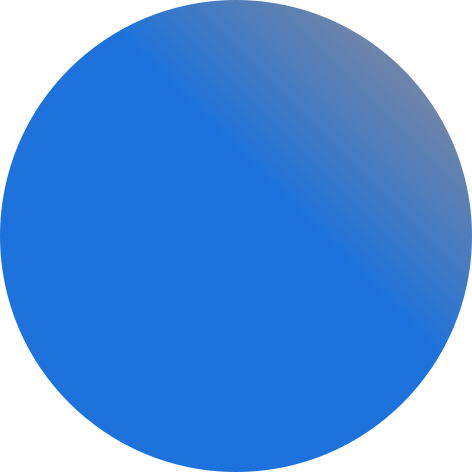
\includegraphics[scale=0.15]{obstacles/fond_bleu}, 
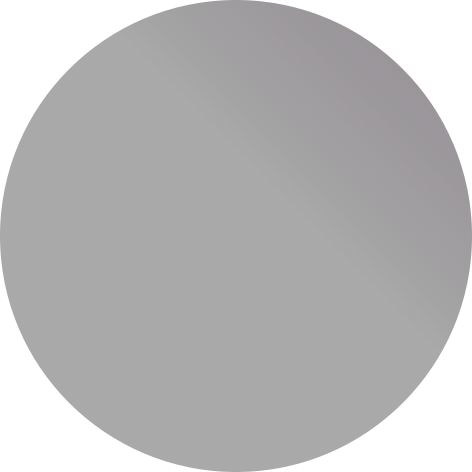
\includegraphics[scale=0.15]{obstacles/fond_gris}, 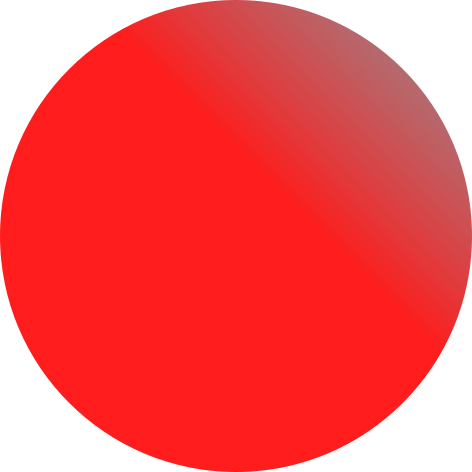
\includegraphics[scale=0.15]{obstacles/fond_rouge}, 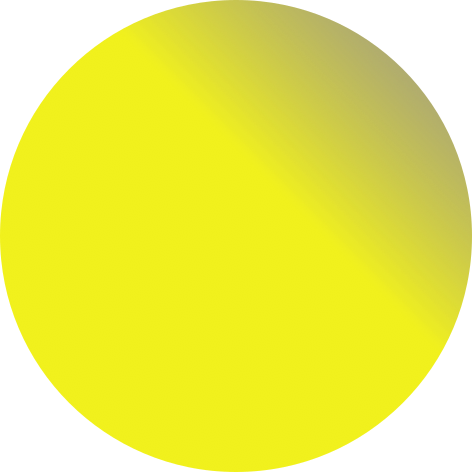
\includegraphics[scale=0.15]{obstacles/fond_jaune}, 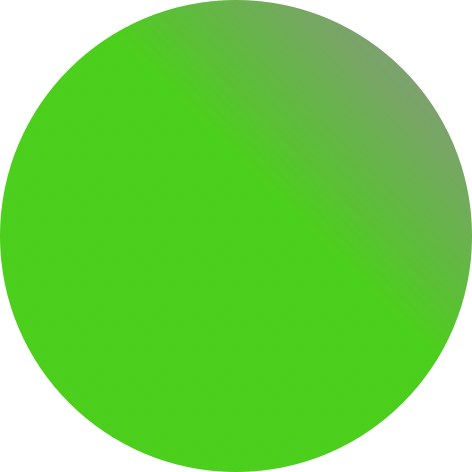
\includegraphics[scale=0.15]{obstacles/fond_vert}, 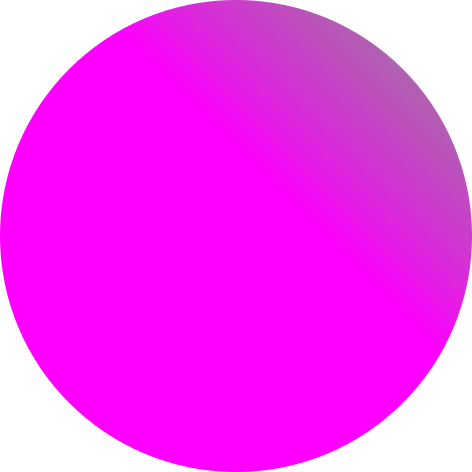
\includegraphics[scale=0.15]{obstacles/fond_violet} ). D'un côté des valeurs, de l'autre des obstacles. Les valeurs rapportent des points directement, les obstacles en fin de partie.
\item 3x \marqueursObstacles, avec les différents obstacles que vous pouvez rencontrer (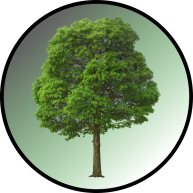
\includegraphics[scale=0.15]{icones/icones_arbre},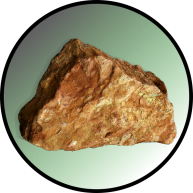
\includegraphics[scale=0.15]{icones/icones_rocher}, 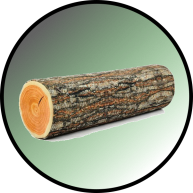
\includegraphics[scale=0.15]{icones/icones_tronc})
\item 15x \jetonsMeteo, qui permettent de mesurer le temps qui passe.
\item 6x randonneurs, avec des couleur différentes (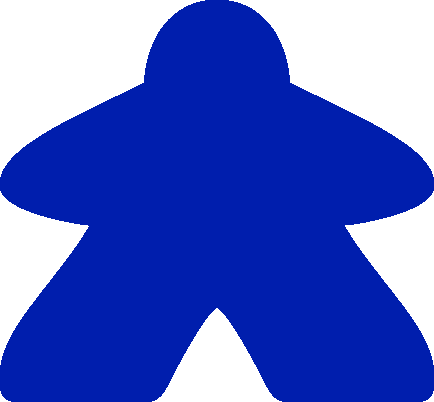
\includegraphics[scale=0.08]{meeples/meepleBleu}, \includegraphics[scale=0.08]{meeples/meepleGRis}, 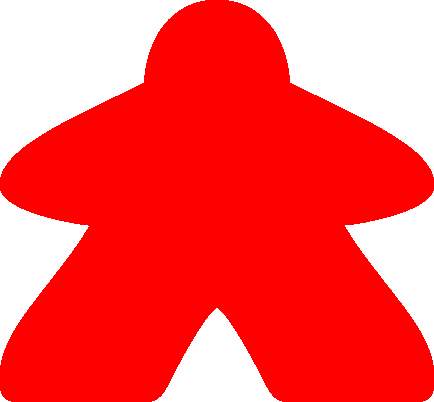
\includegraphics[scale=0.08]{meeples/meepleRouge}, 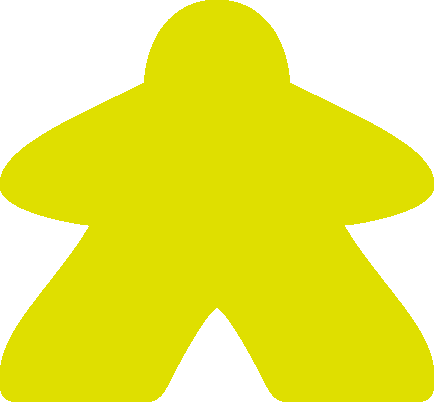
\includegraphics[scale=0.08]{meeples/meepleJaune}, 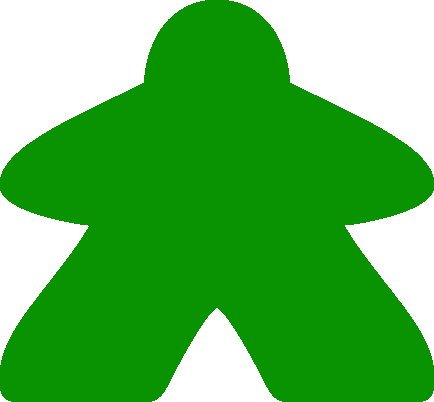
\includegraphics[scale=0.08]{meeples/meepleVert}, 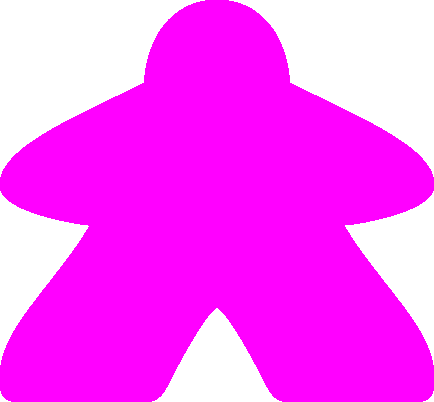
\includegraphics[scale=0.08]{meeples/meepleViolet})
\item 66x cartes recto-verso 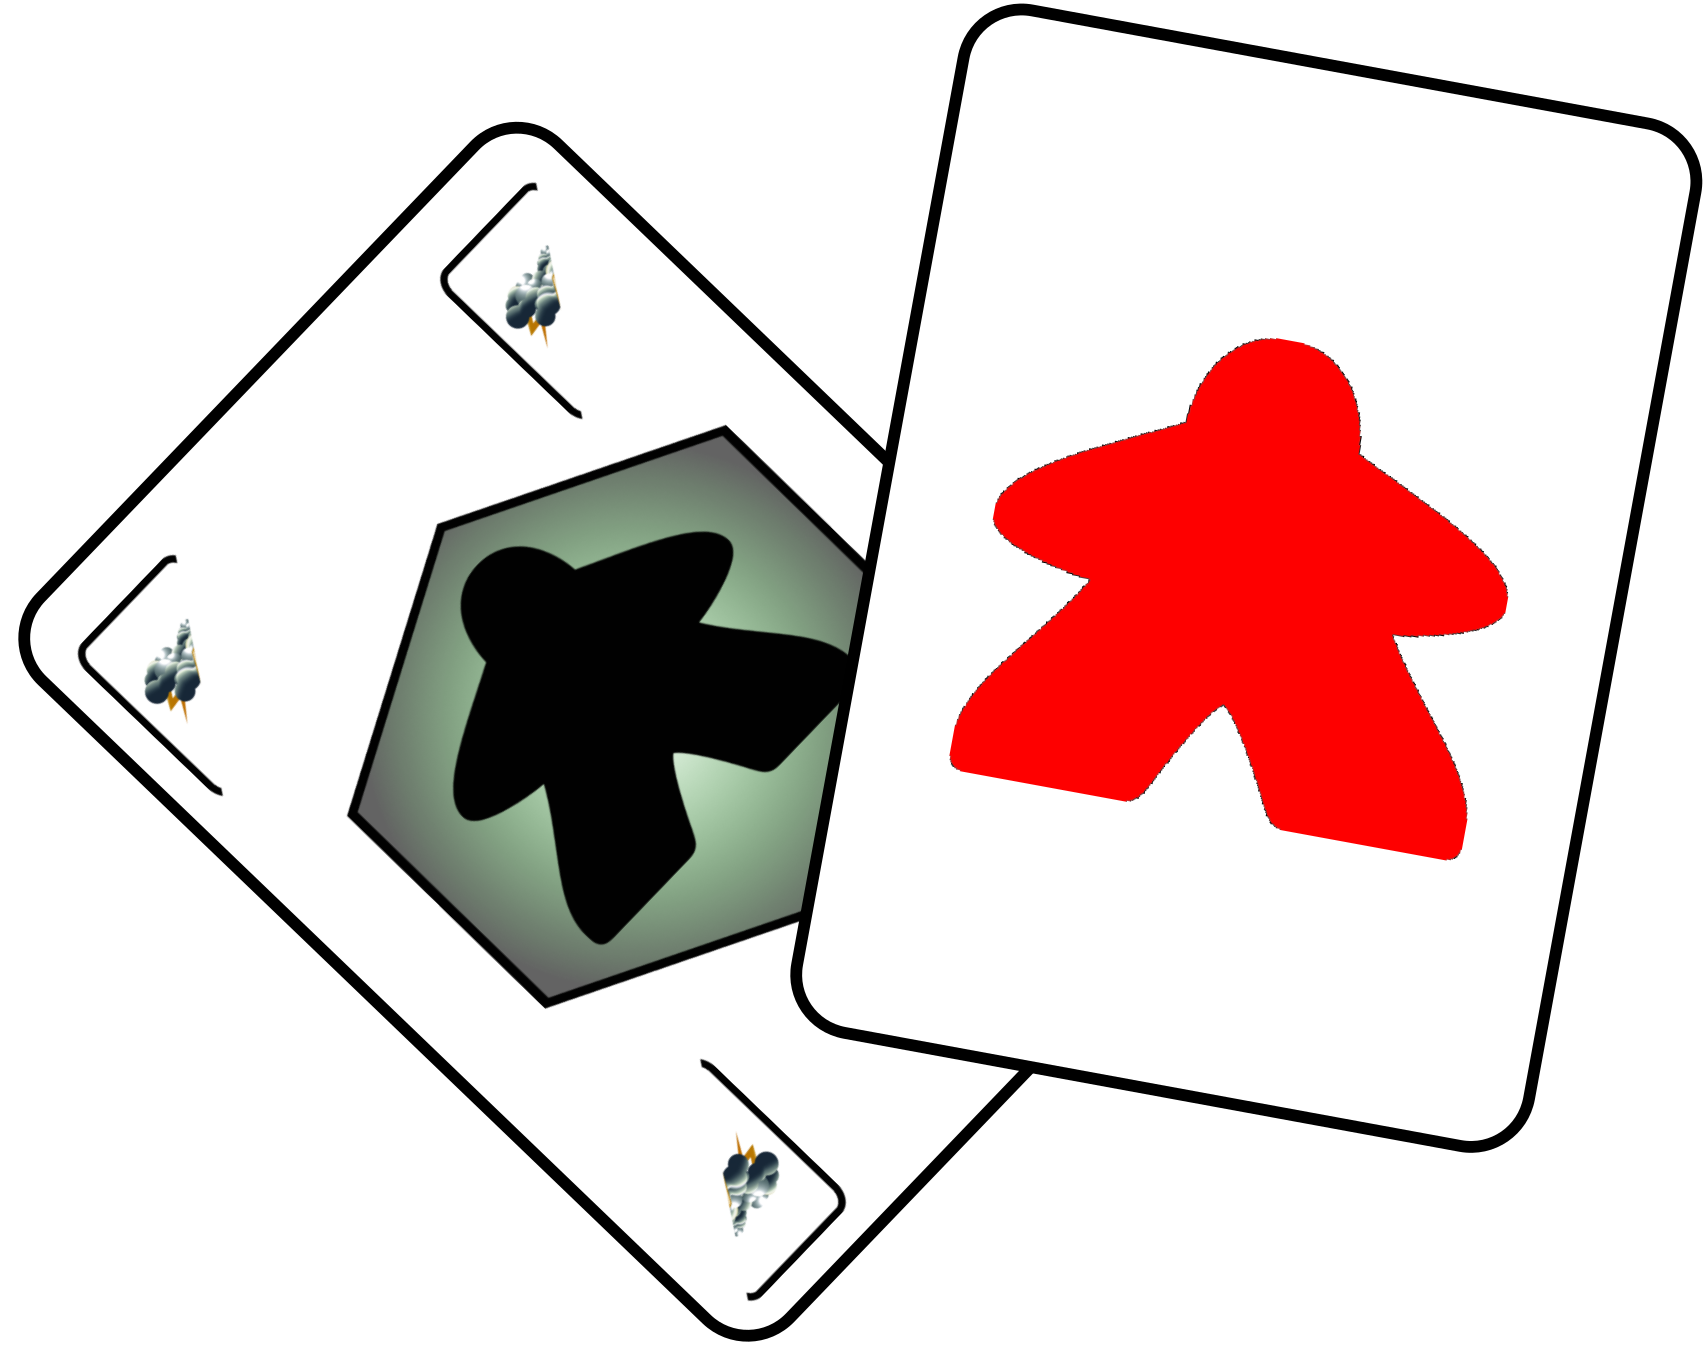
\includegraphics[scale=0.15]{regle/cartes}. D'un côté, des randonneurs, de l'autres de bonus.
\item un plateau central, divisé en plusieurs zones.
\end{itemize}

De plus, chaque joueur possède:
\begin{itemize}
\item un plateau pour indiquer les multiplicateurs d'actions.
\item 9 jetons de son esprit
\item 6 tuiles recto-verso 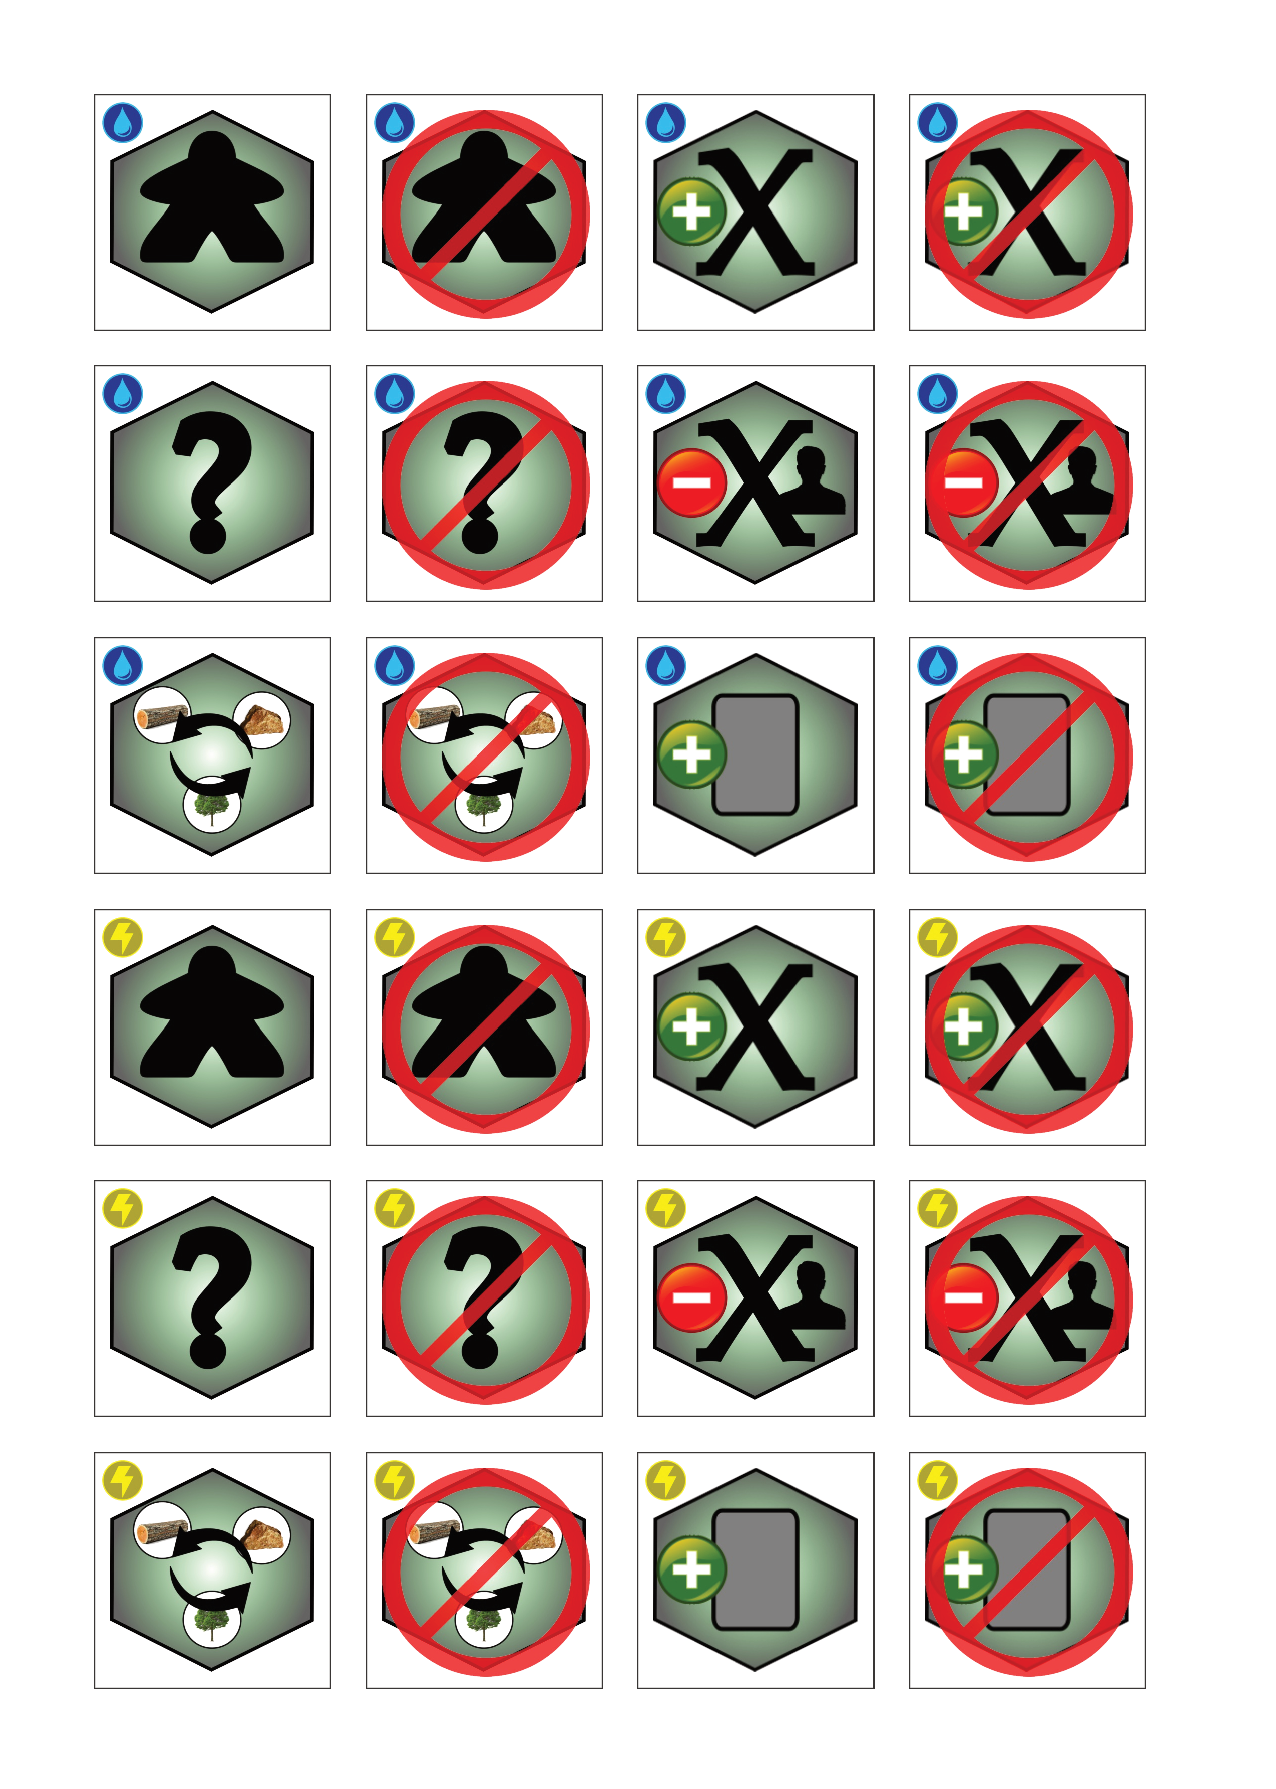
\includegraphics[scale=0.25]{regle/tuiles}, une pour chaque action possible. D'un côte, l'action est accessible (\tuileActive), de l'autre l'action est bloquée (\tuileBloquee).
\end{itemize}
\FloatBarrier
